% !BIB program = biber
\documentclass[11pt]{article}
\usepackage[utf8]{inputenc}	% Para caracteres en español
\usepackage{caption}
\usepackage[backend=biber]{biblatex}
\usepackage{amsmath,amsthm,amsfonts,amssymb,amscd}
\usepackage{multirow,booktabs}
\usepackage[table]{xcolor}
\usepackage{graphicx}
\usepackage{fullpage}
% \usepackage{lastpage}
\usepackage{enumitem}
\usepackage{pgfplots}
\pgfplotsset{compat=1.18}
\usepackage{fancyhdr}
\usepackage{mathrsfs}
\usepackage{fancyhdr}
\setlength{\headheight}{14pt}
\usepackage{wrapfig}
\usepackage{setspace}
\usepackage{calc}
\usepackage{multicol}
\usepackage{cancel}
\usepackage{tikz}
\usetikzlibrary{positioning}
\usepackage[retainorgcmds]{IEEEtrantools}
\usepackage[margin=3cm]{geometry}
\usepackage{amsmath}
\newlength{\tabcont}
\setlength{\parindent}{0.0in}
\setlength{\parskip}{0.05in}
\usepackage{empheq}
\usetikzlibrary{intersections}
\usepackage{framed}
\usepackage[most]{tcolorbox}
\usepackage{xcolor}
\usepackage[ruled,vlined]{algorithm2e}
\colorlet{shadecolor}{orange!15}
\parindent 0in
\parskip 12pt
\usepgfplotslibrary{groupplots}
\geometry{margin=1in, headsep=0.25in}
\theoremstyle{definition}
\newtheorem{defn}{Definition}
\newtheorem{definition}{Definition}
\newtheorem{reg}{Rule}
\newtheorem{exer}{Exercise}
\newtheorem{note}{Note}  % Numbered Note
\newtheorem*{unnote}{Note}  % Unnumbered Note
\newtheorem{mynote}{Note:}  % Numbered Note:
\newtheorem*{myunnote}{Note:} % Unnumbered Note:
\thispagestyle{empty}
\pagestyle{fancy}
\fancyhf{}
\addbibresource{ComputerVision.bib}
\begin{document}
\section*{PROBLEM 1 (10 points = 4 + 6)}

Given a 2-D Gaussian smoothing filter of the form
\begin{equation}
G(x,y;\sigma)=\frac{1}{2\pi\sigma^{2}}\exp\left(-\frac{(x^{2}+y^{2})}{2\sigma^{2}}\right)
\end{equation}

(a) Explain briefly why the Gaussian smoothing filter is considered optimal. How does the choice of the $\sigma$ value for the Gaussian smoothing filter affect the result of the smoothing process? (4 points)

(b) Show that the 2-D Gaussian smoothing filter is separable. Also show how the separability of the 2-D Gaussian filter can result in computational savings for an $N \times N$ image processed with a Gaussian filter of size $M \times M$ where $M < N$. You are expected to derive the order of complexity (big-Oh) of the filtering operation in terms of $N$ and $M$ in each case: (6 points)

\begin{enumerate}[label=(\roman*)]
    \item 2-D Gaussian filter is not separated.
    \item 2-D Gaussian filter is separated into two 1-D filters.
\end{enumerate}

\vspace{1cm}
\newpage
\section*{PROBLEM 2 (10 points = 2 + 2 + 6)}

\begin{center}
    \begin{tikzpicture}
        \begin{groupplot}[
            group style={
                group size=2 by 1, % 2 columns, 1 row
                horizontal sep=2cm, % Clear separation between plots
            },
            width=7cm, height=6cm,
            axis x line=middle, 
            axis y line=middle,
            xmin=-5, xmax=5,
            ymin=-1.2, ymax=1.2,
            ticks=none,
            xlabel={}, ylabel={},
            every axis x label/.style={at={(current axis.right of origin)},anchor=west},
            every axis y label/.style={at={(current axis.above origin)},anchor=south},
        ]
            % LEFT PLOT: LoG Operator (Mexican Hat)
            \nextgroupplot[title={1-D LoG Operator}]
            \addplot[thick, samples=100, domain=-4.5:4.5] { (1 - x^2) * exp(-x^2/2) };
            
            % RIGHT PLOT: Response to a Step Edge
            \nextgroupplot[title={Response to Step Edge}]
            % The response to a step edge is the first derivative of the Gaussian
            \addplot[thick, samples=100, domain=-4.5:4.5] { -x * exp(-x^2/2) };
        \end{groupplot}
    \end{tikzpicture}
    \captionof{figure}{LoG operator and its response to a step edge}
\end{center}


(a) Shown in Figure 1 is a 1-D Laplacian-of-Gaussian (LoG) operator with width $\sigma=2$ and the result of convolving the operator with a step edge of a given magnitude (height). Sketch the 1-D LoG operators with width $\sigma=1$ and $\sigma=3$ and the corresponding outputs resulting from convolving them with the same step edge. (2 points)

(b) Show that the 2-D LoG is rotationally symmetric. (2 points)

(c) Outline a computationally efficient way of implementing the 2-D LoG operator. Show the computational advantage in doing so over the straightforward implementation of the 2-D LoG operator using big-Oh analysis for both implementations. (6 points)

\newpage

\section*{PROBLEM 3 (20 points = 3 + 8 + 3 + 3 + 3)}

(a) What is the advantage of multi-scale edge detection over single-scale edge detection using the LoG operator? (3 points)

(b) Give an outline of the multi-scale edge detection algorithm by Bergholm. (8 points)

(c) Give a justification for the value of step size $\Delta\sigma \le 0.5$ between successive scales. (3 points)

(d) How would a larger value of $\Delta\sigma$ affect the output of the algorithm? (3 points)

(e) What is the role of the non-maxima suppression technique in the Canny edge detector. Why it is necessary? (3 points)

\vspace{1cm}

\section*{PROBLEM 4 (20 points = 6 + 11 + 3)}

You are given an $N$ by $N$ edge image with $E$ edge pixels (fragments).

(a) Outline the Hough Transform algorithm to detect circles in this edge image assuming that the edge pixels do not contain local gradient direction information. Determine the memory requirement and run-time complexity of this algorithm using the big-Oh notation. (6 points)

(b) Outline the Hough Transform algorithm to detect circles in this edge image assuming that the edge fragments contain local gradient direction information. Determine the memory requirement and run-time complexity of this algorithm using the big-Oh notation. What is the advantage of using gradient direction information in terms of memory requirement and run-time complexity? (11 points)

(c) Why is the polar equation of the line $\rho = x \cos \theta + y \sin \theta$ preferred over the Cartesian equation of the line $y = mx + c$ when using the Hough Transform for line detection? (3 points)

\newpage

\section*{PROBLEM 5 (20 points = 8 + 12)}


\begin{center}
    \begin{minipage}{0.6\textwidth}
        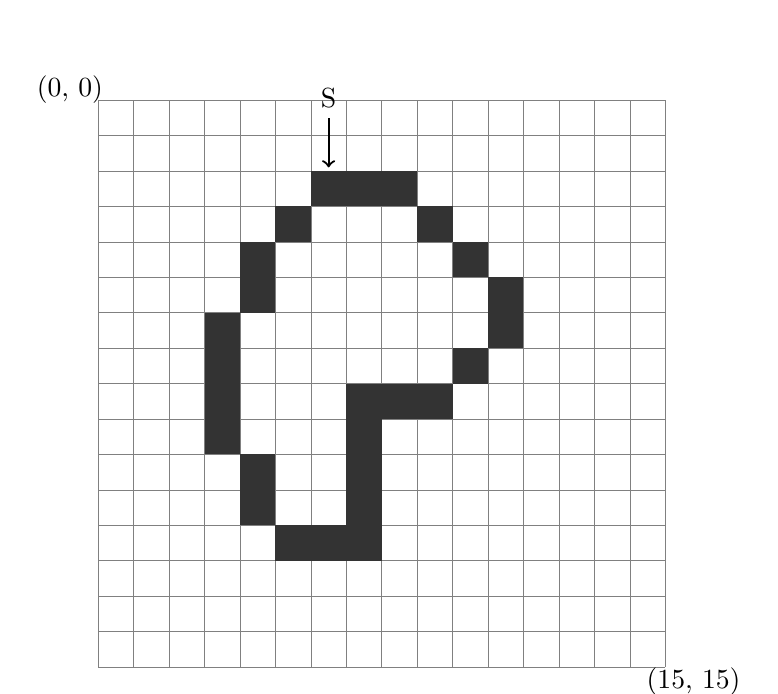
\begin{tikzpicture}[scale=0.45]
            % Draw the 16x16 grid
            \draw[step=1cm, gray, very thin] (0,0) grid (16,16);
            
            % Coordinate Labels
            \node at (-0.8, 16.3) {(0, 0)};
            \node at (16.8, -0.4) {(15, 15)};
            
            % --- SHAPE CONTOUR ---
            % Top Bar
            \fill[black!80] (6,13) rectangle (9,14); 
            
            % Right Side
            \fill[black!80] (9,12) rectangle (10,13);
            \fill[black!80] (10,11) rectangle (11,12);
            \fill[black!80] (11,9) rectangle (12,11); % 2 blocks vertical
            \fill[black!80] (10,8) rectangle (11,9);
            
            % Inner Notch (Right-Bottom)
            \fill[black!80] (7,7) rectangle (10,8);  % Horizontal notch segment
            \fill[black!80] (7,4) rectangle (8,7);   % Vertical notch segment (3 blocks down)
            
            % Bottom Bar
            \fill[black!80] (5,3) rectangle (8,4);
            
            % Left Side
            \fill[black!80] (4,4) rectangle (5,6);   % 2 blocks vertical (bottom-left curve)
            \fill[black!80] (3,6) rectangle (4,10);  % 4 blocks vertical (main left edge)
            \fill[black!80] (4,10) rectangle (5,12); % 2 blocks vertical (top-left curve)
            \fill[black!80] (5,12) rectangle (6,13);
            
            % Arrow and 'S' Label
            % Pointing exactly to the center of the first block of the top bar (x=6.5)
            \draw[<-, thick] (6.5, 14.1) -- (6.5, 15.5) node[above] {S};
            
        \end{tikzpicture}
    \end{minipage}
    \begin{minipage}{0.3\textwidth}
        \centering
        \begin{tabular}{|c|c|c|}
            \hline 1 & 2 & 3 \\ \hline
            0 & $\times$ & 4 \\ \hline
            7 & 6 & 5 \\ \hline
        \end{tabular}
        \\[5pt] Direction codes
    \end{minipage}
    \captionof{figure}{Contour for chain code}
\end{center}



(a) For Figure 2 give the chain code for the contour starting from pixel S and traversing the contour in the clockwise direction. Use the direction codes indicated in Figure 2. What would be the corresponding $1^{st}$-difference chain code be for the same contour? (8 points)

(b) Why are $1^{st}$-difference chain codes useful for contour-based recognition of 2-D objects? Outline a algorithm that would perform contour-based 2-D object recognition using differential chain codes. Assume you have a single object in the image and $N$ objects in the model database. (12 points)

\vspace{1cm}

\section*{PROBLEM 6 (20 points = 16 + 4)}

(a) Outline a scheme to recognize an arbitrary 2-D shape in an image using the generalized Hough transform. Assume that the 2-D shape has 4 degrees of freedom in the image (i.e., two translation parameters, one rotation parameter and one scale parameter). (16 points)

(b) How would you modify the scheme in (a) above to detect only moving (i.e., dynamic) instances of the 2-D shape in each image frame? (4 points)



0,0,0,0,0,0,0,0,0,0,0,0,0,0,0,0,
0,0,0,0,0,0,0,0,0,0,0,0,0,0,0,0,
0,0,0,0,0,0,1,1,1,0,0,0,0,0,0,0,
0,0,0,0,0,1,0,0,0,1,0,0,0,0,0,0,
0,0,0,0,0,1,0,0,0,0,1,0,0,0,0,0,
0,0,0,0,1,0,0,0,0,0,0,1,0,0,0,0,
0,0,0,1,0,0,0,0,0,0,0,1,0,0,0,0,
0,0,0,1,0,0,0,0,0,0,1,0,0,0,0,0,
0,0,0,1,0,0,0,1,1,1,0,0,0,0,0,0,
0,0,0,1,0,0,0,1,0,0,0,0,0,0,0,0,
0,0,0,0,1,0,0,1,0,0,0,0,0,0,0,0
0,0,0,0,1,1,1,0,0,0,0,0,0,0,0,0
0,0,0,0,0,0,0,0,0,0,0,0,0,0,0,0,
0,0,0,0,0,0,0,0,0,0,0,0,0,0,0,0,
0,0,0,0,0,0,0,0,0,0,0,0,0,0,0,0,
0,0,0,0,0,0,0,0,0,0,0,0,0,0,0,0,
\end{document}
